\documentclass[notes xcolor=dvipsnames]{beamer}

\usetheme{Berkeley}

\usepackage{amsmath}
\usepackage{graphicx}

\title{Scheduling Weakly Consistent C Programs for Reconfigurable Hardware}
\subtitle{Nadesh Ramanathan, John Wickerson, George Constantinides.}

\author{Presented by \\ Akshay Gopalakrishnan}

\begin{document}
    
    \begin{frame}

        \maketitle

    \end{frame}

    \begin{frame}{Who are they?}

    \end{frame}

    \section{Introduction}
    \begin{frame}{Example}

        %Put a set of questions here that this work is trying to answer
        \begin{columns}
            
            \begin{column}{0.5\textwidth}
                \begin{figure}
                    \makebox[\textwidth][c]{
                        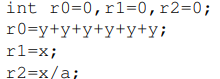
\includegraphics[scale=0.7]{RR-Part1.PNG}
                    }
                \end{figure}
                
            \end{column}

            \begin{column}{0.5\textwidth}

                \begin{figure}
                    \makebox[\textwidth][c]{
                        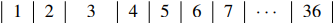
\includegraphics[scale=0.7]{RR-cycles.PNG}
                    }
                \end{figure}

                \begin{figure}
                    \makebox[\textwidth][c]{
                        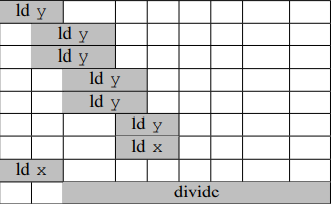
\includegraphics[scale=0.7]{RR-sched-part1.PNG}
                    }
                \end{figure}
                
            \end{column}


        \end{columns}
        
        

    \end{frame}

    \begin{frame}{Example}

        %Put a set of questions here that this work is trying to answer
        \begin{columns}
            
            \begin{column}{0.5\textwidth}
                \begin{figure}
                    \makebox[\textwidth][c]{
                        
\includegraphics[scale=0.7]{RR-part2.PNG}
                    }
                \end{figure}
                
            \end{column}

            \begin{column}{0.5\textwidth}

                \begin{figure}
                    \makebox[\textwidth][c]{
                        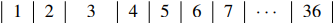
\includegraphics[scale=0.7]{RR-cycles.PNG}
                    }
                \end{figure}

                \begin{figure}
                    \makebox[\textwidth][c]{
                        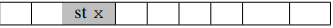
\includegraphics[scale=0.7]{RR-sched-part2.PNG}
                    }
                \end{figure}
                
            \end{column}


        \end{columns}
        
        

    \end{frame}


    \begin{frame}{Example}

        %Put a set of questions here that this work is trying to answer
        \begin{columns}
            
            \begin{column}{0.5\textwidth}
                \begin{figure}
                    \makebox[\textwidth][c]{
                        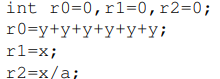
\includegraphics[scale=0.7]{RR-Part1.PNG}
                    }
                \end{figure}

                \begin{figure}
                    \makebox[\textwidth][c]{
                        \includegraphics[scale=0.7]{RR-Part2.PNG}
                    }
                \end{figure}

                \begin{figure}
                    \makebox[\textwidth][c]{
                        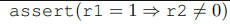
\includegraphics[scale=0.7]{RR-assert.PNG}
                    }
                \end{figure}

                
            \end{column}

            \begin{column}{0.5\textwidth}
                
                \begin{figure}
                    \makebox[\textwidth][c]{
                        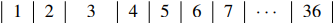
\includegraphics[scale=0.7]{RR-cycles.PNG}
                    }
                \end{figure}

                
                \begin{figure}
                    \makebox[\textwidth][c]{
                        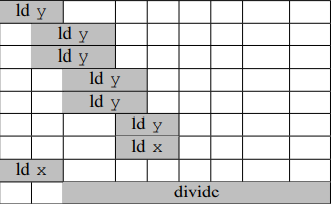
\includegraphics[scale=0.7]{RR-sched-part1.PNG}
                    }
                \end{figure}

                \begin{figure}
                    \makebox[\textwidth][c]{
                        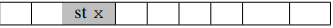
\includegraphics[scale=0.7]{RR-sched-part2.PNG}
                    }
                \end{figure}
                
            \end{column}


        \end{columns}
        
        

    \end{frame}

    %Example 2
    \begin{frame}{Example}

        %Put a set of questions here that this work is trying to answer
        \begin{columns}
            
            \begin{column}{0.5\textwidth}
                \begin{figure}
                    \makebox[\textwidth][c]{
                        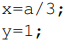
\includegraphics[scale=0.7]{WW-part1.PNG}
                    }
                \end{figure}
                
            \end{column}

            \begin{column}{0.5\textwidth}

                \begin{figure}
                    \makebox[\textwidth][c]{
                        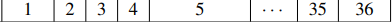
\includegraphics[scale=0.7]{WW-cycles.PNG}
                    }
                \end{figure}

                \begin{figure}
                    \makebox[\textwidth][c]{
                        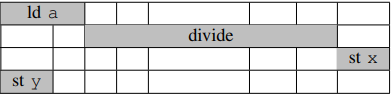
\includegraphics[scale=0.7]{WW-sched-part1.PNG}
                    }
                \end{figure}
                
            \end{column}


        \end{columns}
        
        

    \end{frame}

    \begin{frame}{Example}

        %Put a set of questions here that this work is trying to answer
        \begin{columns}
            
            \begin{column}{0.5\textwidth}
                \begin{figure}
                    \makebox[\textwidth][c]{
                        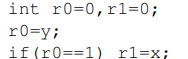
\includegraphics[scale=0.7]{WW-part2.PNG}
                    }
                \end{figure}
                
            \end{column}

            \begin{column}{0.5\textwidth}

                \begin{figure}
                    \makebox[\textwidth][c]{
                        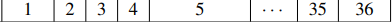
\includegraphics[scale=0.7]{WW-cycles.PNG}
                    }
                \end{figure}

                \begin{figure}
                    \makebox[\textwidth][c]{
                        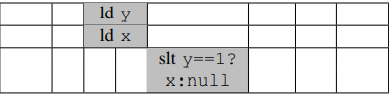
\includegraphics[scale=0.7]{WW-sched-part2.PNG}
                    }
                \end{figure}
                
            \end{column}


        \end{columns}
        
        

    \end{frame}


    \begin{frame}{Example}

        %Put a set of questions here that this work is trying to answer
        \begin{columns}
            
            \begin{column}{0.5\textwidth}
                \begin{figure}
                    \makebox[\textwidth][c]{
                        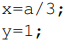
\includegraphics[scale=0.7]{WW-part1.PNG}
                    }
                \end{figure}

                \begin{figure}
                    \makebox[\textwidth][c]{
                        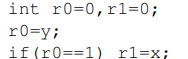
\includegraphics[scale=0.7]{WW-part2.PNG}
                    }
                \end{figure}

                \begin{figure}
                    \makebox[\textwidth][c]{
                        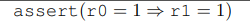
\includegraphics[scale=0.7]{WW-assert.PNG}
                    }
                \end{figure}
                
            \end{column}

            \begin{column}{0.5\textwidth}
                
                \begin{figure}
                    \makebox[\textwidth][c]{
                        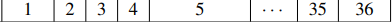
\includegraphics[scale=0.7]{WW-cycles.PNG}
                    }
                \end{figure}

                
                \begin{figure}
                    \makebox[\textwidth][c]{
                        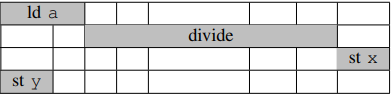
\includegraphics[scale=0.7]{WW-sched-part1.PNG}
                    }
                \end{figure}

                \begin{figure}
                    \makebox[\textwidth][c]{
                        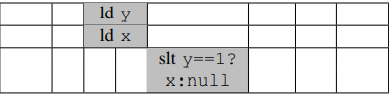
\includegraphics[scale=0.7]{WW-sched-part2.PNG}
                    }
                \end{figure}
                
            \end{column}


        \end{columns}
        
        

    \end{frame}

    \begin{frame}{Problem of Dependencies}


        \begin{figure}
            \makebox[\textwidth][c]{
                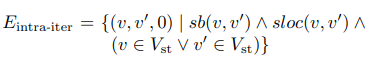
\includegraphics{IntraIter-Dep.PNG}
            }
        \end{figure}

        \begin{figure}
            \makebox[\textwidth][c]{
                \includegraphics{InterIter-Dep.PNG}
            }
        \end{figure}
        
    \end{frame}

   

    \begin{frame}{Adding WW|WR|RW|RR Dependancies}

        \begin{figure}
            \makebox[\textwidth][c]{
                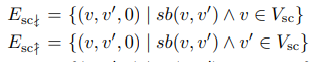
\includegraphics{SC-constraint.PNG}
            }
        \end{figure}

        \begin{columns}
            
            \begin{column}{0.5\textwidth}

                \begin{figure}
                    \makebox[\textwidth][c]{
                        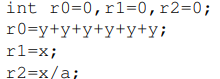
\includegraphics{RR-Part1.PNG}
                    }
                \end{figure}
                
            \end{column}

            \begin{column}{0.5\textwidth}
                
                \begin{figure}
                    \makebox[\textwidth][c]{
                        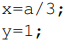
\includegraphics{WW-part1.PNG}
                    }
                \end{figure}

            \end{column}

        \end{columns}
        
    \end{frame}

    \begin{frame}{Final Dependency Expression}

        \begin{figure}
            \makebox[\textwidth][c]{
                \includegraphics{Strong-constraint.PNG}
            }
        \end{figure}
        
    \end{frame}
    


    \begin{frame}{Example}

        Without pipelining
        \begin{figure}
            \makebox[\textwidth][c]{
                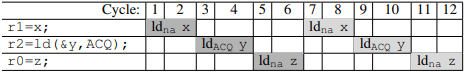
\includegraphics[scale=0.7]{Gen-ex-SC-no-pipe.PNG}
            }
        \end{figure}
             
        With pipelining
        \begin{figure}
            \makebox[\textwidth][c]{
                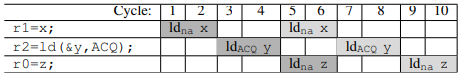
\includegraphics[scale=0.7]{Gen-ex-SC-pipe.PNG}
            }
        \end{figure}     
        
    \end{frame}

    \begin{frame}{Weakening: Adding Release-Acquire Dependencies}
        
        \begin{figure}
            \makebox[\textwidth][c]{
                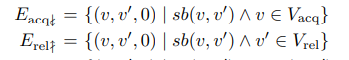
\includegraphics{Rel-Acq-Constraint.PNG}
            }
        \end{figure}

        
        \begin{columns}
            
            \begin{column}{0.5\textwidth}

                \begin{figure}
                    \makebox[\textwidth][c]{
                        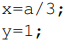
\includegraphics{WW-part1.PNG}
                    }
                \end{figure}
                
            \end{column}

            \begin{column}{0.5\textwidth}
                
                \begin{figure}
                    \makebox[\textwidth][c]{
                        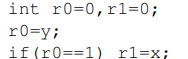
\includegraphics{WW-part2.PNG}
                    }
                \end{figure}

            \end{column}

        \end{columns}
    
    \end{frame}

    \begin{frame}{Adding RR Dependency}

            \begin{figure}
                \makebox[\textwidth][c]{
                    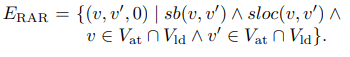
\includegraphics{RR-constraint.PNG}
                }
            \end{figure}
            
            \begin{figure}
                \makebox[\textwidth][c]{
                    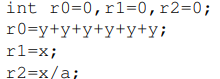
\includegraphics{RR-Part1.PNG}
                }
            \end{figure}
            
            
    \end{frame}

    \begin{frame}{Final Dependency Expression}

        \begin{figure}
            \makebox[\textwidth][c]{
                \includegraphics{Weak-constraint.PNG}
            }
        \end{figure}
        
    \end{frame}

    
    \begin{frame}{Example}

        Without pipelining
        \begin{figure}
            \makebox[\textwidth][c]{
                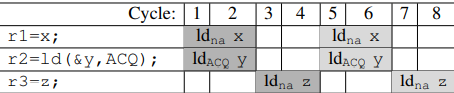
\includegraphics[scale=0.7]{Gen-ex-Acq-no-pipe.PNG}
            }
        \end{figure}
             
        With pipelining
        \begin{figure}
            \makebox[\textwidth][c]{
                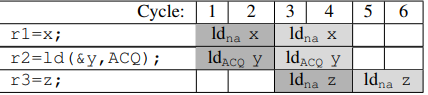
\includegraphics[scale=0.7]{Gen-ex-Acq-pipe.PNG}
            }
        \end{figure}     
        
    \end{frame}

    %TEsting on Message passing algorithm
    \begin{frame}{Testing on Message Passing}

        \begin{figure}
            \makebox[\textwidth][c]{
                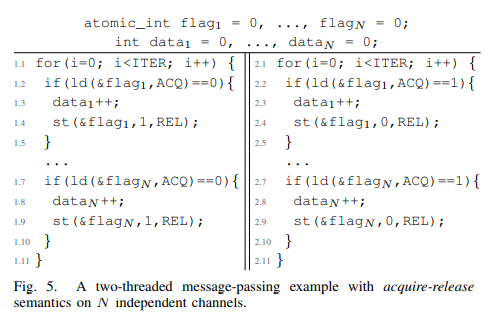
\includegraphics[scale=0.7]{MP-Acq-Rel.PNG}
            }
        \end{figure}
        
    \end{frame}


    \begin{frame}{Testing on Message Passing}

        \begin{figure}
            \makebox[\textwidth][c]{
                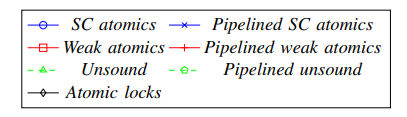
\includegraphics[scale=0.7]{MP-Legend.PNG}
            }
        \end{figure}

        \begin{figure}
            \makebox[\textwidth][c]{
                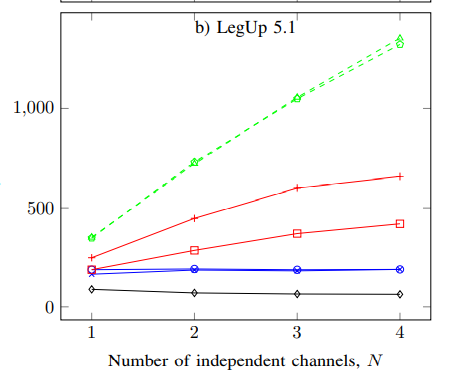
\includegraphics[scale=0.7]{MP_eval.PNG}
            }
        \end{figure}

        
    \end{frame}

    \begin{frame}{Pros and Cons}
        \begin{figure}
            \makebox[\textwidth][c]{
                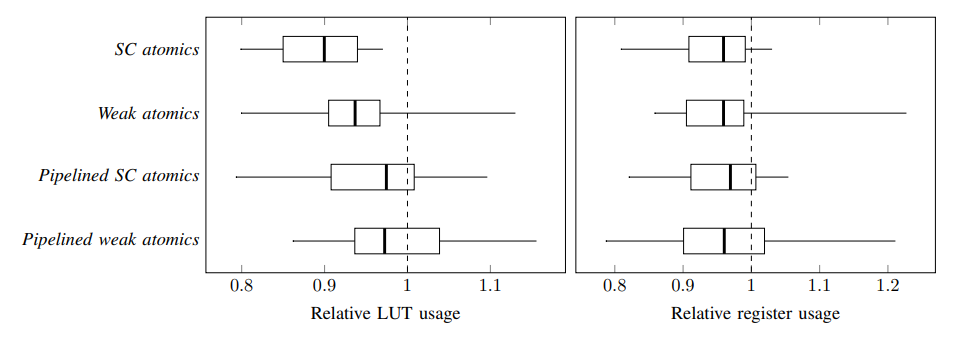
\includegraphics[scale=0.5]{LUT-Reg-Usage.PNG}
            }
        \end{figure}
        
    \end{frame}

    \begin{frame}{Conclusion}

    \end{frame}


\end{document}